\chapter{Background}

\section{Delta-tracking theory}

The delta-tracking method was introduced by Woodcock in the 1960s. Although widely known, the method has
not been commonly used as the primary transport method in general purpose Monte Carlo codes, probably 
because of its limitations discussed below \cite{serp_delta}.

In Monte Carlo neutron transport, we track anything that can happen to neutrons in a system: collisions 
and their outcomes, surface crossings, etc. To do that, we need to track how these particles move in that 
system. This starts with determining the number of path lengths they cover between events.
The number of path lengths traveled by a given neutron is sampled from an exponential distribution using

\begin{equation}
\ell = \frac{-\log\xi}{\Sigma_{\mathrm{tot,m}}(E)},
\end{equation}

\noindent where $\xi$ is a uniformly-distributed random variable on the unit interval and 
$\Sigma_{\mathrm{tot,m}}$ is the macroscopic total cross section of the material $m$ in which the neutron 
is located. The total cross section characterizes the neutron collision probability per unit path length 
traveled in the medium.

However, the sampled path length is not statistically valid if the neutron crosses a material boundary; 
the flight is stopped at the boundary surface and a new path length is sampled with the new material total
cross section. This is the main principle of conventional ray tracing \cite{serp_delta} and is what is
done in WARP with the OptiX framework, as discussed below.

The idea behind delta-tracking is to effectively homogenize the total cross sections such that the sampled
path lengths are valid over the entire geometry. Consider the concept of the ``virtual collision", a 
scattering reaction that preserves neutron energy and direction. Since virtual collisions have no impact 
on the final outcome, any number of them can ``happen" in the random walk. Therefore, the total cross 
section of a material can be adjusted by adding an arbitrary virtual collision cross section, 
$\Sigma_\mathrm{{0,m}}(E)$
\cite{serp_delta}:

\begin{equation}
\Sigma'_{\mathrm{tot,m}}(E) = \Sigma_{\mathrm{tot,m}}(E) + \Sigma_\mathrm{{0,m}}(E).
\end{equation}

Because all material cross sections can now be freely and arbitrarily increased, a \textit{majorant} cross
section can be assigned to represent the effective total (physical + virtual) collision probability in all
materials along a given neutron's trajectory:
\begin{equation}
\label{eq:maj}
\begin{aligned}
\Sigma_{\mathrm{maj}}(E) &= \Sigma'_{\mathrm{tot,1}}(E) = \Sigma'_{\mathrm{tot,2}}(E) = \ldots = 
\Sigma'_{\mathrm{tot,M}}(E) \\
& = \max\{\Sigma_{\mathrm{tot,1}}(E), \Sigma_{\mathrm{tot,2}}(E), \ldots, \Sigma_{\mathrm{tot,M}}(E)\}\:,
\end{aligned}
\end{equation}
where $M$ is the number of materials along a neutron's flight path.

Path lengths sampled using the global majorant are statistically valid in all materials, effectively
homogenizing the material total cross sections and eliminating the need to calculate surface intersection
distances \cite{serp_delta}. Instead, an additional step is included in the tracking routine for handling 
virtual collisions. Rejection sampling is carried out for each collision, and the collision point is 
accepted with probability 

\begin{equation}
P_{\mathrm{col}}(E) = \frac{\Sigma_{\mathrm{tot,col}}(E)}{\Sigma_{\mathrm{maj}}(E)}. 
\end{equation}

\noindent If the point is rejected, the collision is considered virtual and the random walk continues by 
sampling a new path length.

The inherent advantage of delta-tracking is that the neutron random walk can be continued over material
boundaries without stopping the walk at each surface crossing. The geometry routine reduces to
determining the material in which the collision point resides, which is computationally less expensive 
than calculating the surface distances when running a simulation on traditional CPU hardware 
\cite{serp_delta}. The simplified geometry routine is advantageous in that delta-tracking is often faster 
than ray tracing in complex geometries, and complicated objects and surface types are easier to handle 
with a delta-tracking algorithm \cite{serp_delta}.

One shortcoming of the delta-tracking method arises when material total cross sections differ greatly. A
representative example of this is a light water reactor (LWR) fuel assembly that contains localized heavy 
absorbers (such as control rods or burnable poison rods) \cite{serp_delta}. Although the absorber itself
occupies a relatively small space physically, its large cross section dominates the majorant at low 
neutron energies. This causes the neutron random walk to be cut into many short tracks, wasting computing
time by continually incurring virtual collisions and resampling. 

Additionally, using the delta-tracking method necessitates the use of the collision flux estimator rather 
than the track-length flux estimator, which is generally considered a drawback for implementation in 
traditional Monte Carlo codes \cite{serp_delta}. The track-length estimation of the reaction rate integral
can be written in simplest analog form as

\begin{equation}
R_{\mathrm{tle}} = \sum_{i=1}^{I}\ell_{i}f_{i},
\end{equation}

\noindent where $\ell$ is the neutron track length, $f$ is the response function, and the summation is 
over all tracks in the region of interest. This estimator cannot be used when employing the delta-tracking
method because the sampled neutron paths may extend over several material regions and the discontinuity
points are not known \cite{serp_delta}. 

An alternative to the track-length flux estimator is the collision flux estimator:

\begin{equation}
R_{\mathrm{cfe}} = \sum_{i=1}^{I}\frac{f_i}{\Sigma_{\mathrm{tot,i}}},
\end{equation}

\noindent where $\Sigma_{\mathrm{tot}}$ is the material total macroscopic cross section at the collision 
site and the summation is over all collisions within the region of interest \cite{serp_delta}. This flux 
estimator is problematic in that it often results in poor efficiency for tallies scored in regions of low 
volume or with low collision density. However, the use of the collision flux estimator should not be 
considered a disadvantage for the implementation of the delta-tracking method in WARP; this estimator is 
already the code's flux tally method \cite{warp2015}.

In WARP, the flux tally kernel scores collisions in cell $j$ with volume $V_j$ as shown in Equation 
\ref{tally}, where $\Sigma_{\mathrm{tot,j}}(E)$ is the total macroscopic cross section at energy 
$E_i < E < E_{i+1}$ and $N_{i,j}$ is the number of collisions in that volume \cite{warp2015}:

\begin{equation}
\label{tally}
\bar{\phi}_{i,j} = \frac{1}{V_j}\sum_{i=1}^{N_{i,j}}\frac{1}{\Sigma_{\mathrm{tot,j}}(E)}\:.
\end{equation}

\section{Ray tracing in WARP}
\label{sec:rt}

WARP uses the NVIDIA OptiX ray tracing framework for geometry representation \cite{warp2015}. OptiX is a
highly-optimized, scalable framework developed by NVIDIA for building ray tracing-based applications. It
allows for user-written applications that use ray tracing for graphics, collision detection, and other
fields of interest \cite{optix_man}; the flexibility of the framework makes it suitable for this 
application in Monte Carlo neutron transport. The OptiX engine is composed of a host-based API that 
defines ray tracing based data structures, which works in combination with a CUDA C-based programming 
system that can produce new rays, intersect rays with surfaces, and respond to those intersections 
\cite{optix_man}.

In WARP and other Monte Carlo codes that use ray tracing to track particle locations, material information
is updated when a sampled interaction distance is greater than the nearest surface distance. The neutron 
is moved to the boundary that it will cross, the material information is updated to the material that the 
neutron is entering, and the interaction distance is resampled in the new material using the same 
direction of flight \cite{warp2015}. WARP uses an algorithm that uses the OptiX framework to perform the 
ray tracing required to determine the entering material. Since all of the system geometric information is 
stored in the OptiX context \cite{warp2015}, this allows the material information update to be done 
readily. 

WARP represents geometric volumes as the intersection of the space inside of a given cell with the space
outside any cells that are nested inside of it \cite{warp2015}. For example, if two objects were 
designated to be centered at the same coordinate point with the inner object entirely encompassed by the 
outer object, the space between the two objects would belong to the outer object while the volume inside 
of the inner object would all belong to the inner object. This is important to note because it sets the
type of algorithms that can be used for geometry handling.

WARP's material query algorithm is shown in Figure \ref{whereami} \cite{warp2015}. A list of surface
intersections, ordered by proximity, is generated by iteratively ray tracing along a neutron's direction
of flight and adding the closest surface number to the hit list each time. Tracing is stopped once the
ray hits a predefined outer cell that contains all other cells \cite{warp2015}. Because all surfaces are
closed, the ray intersects any cell surface twice if its origin is not nested in the cell in which the ray
originated. When the list of surface intersections is created, the double entries are removed, resulting 
in a list of cells in which the neutron is nested. The first entry of the list is the cell in which the 
neutron is located at the time of the material query and the second entry of the list is the cell that the
neutron is entering \cite{warp2015}.

\begin{figure}[h!] 
  \centering
    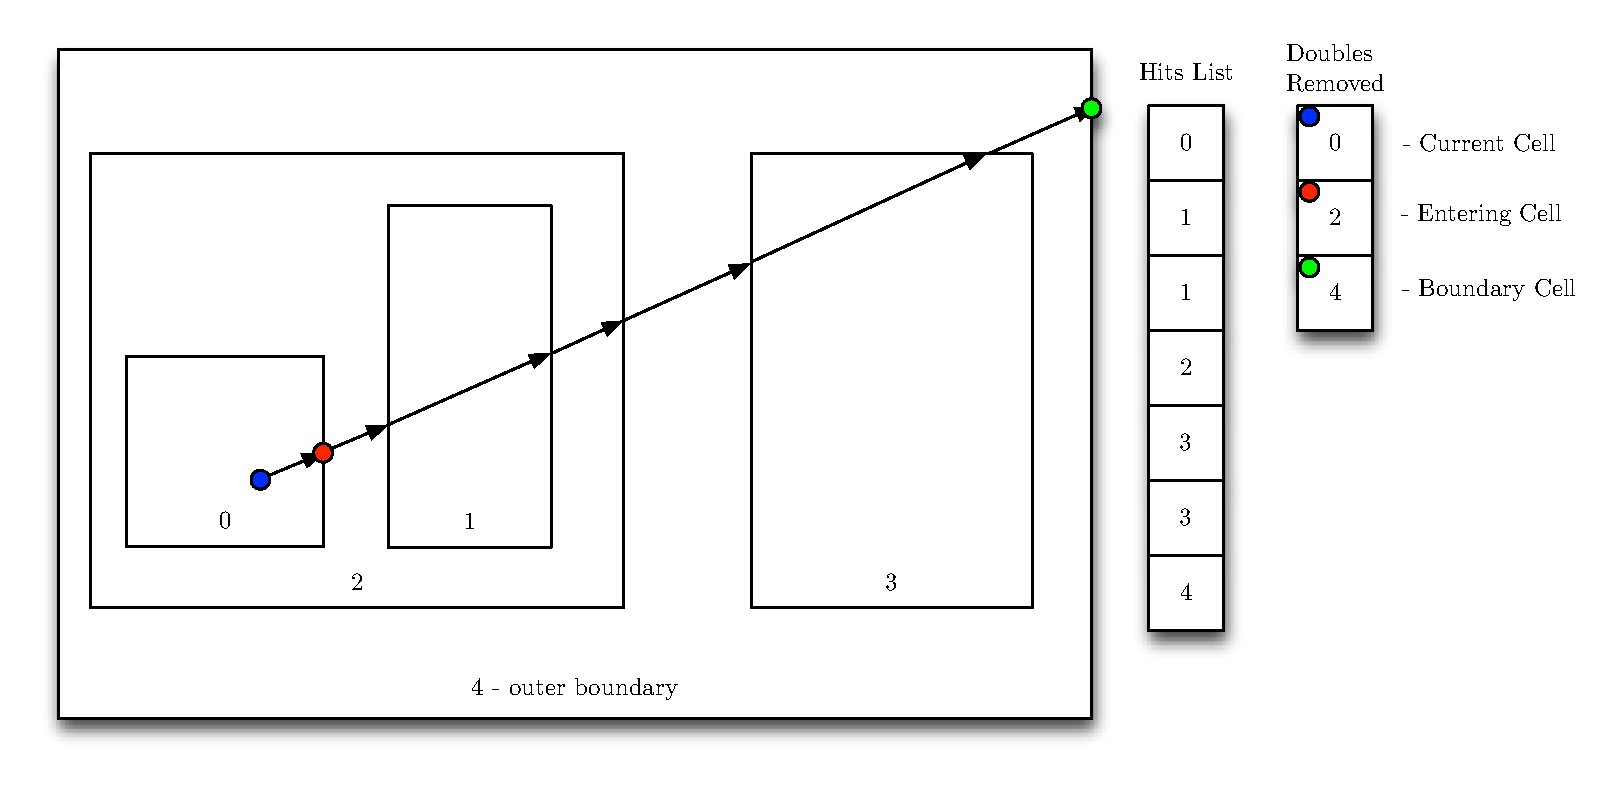
\includegraphics[width=1.0\textwidth]{img/whereami.eps}
     \caption{The point-in-polygon-like algorithm for determining the entering cell/material number by 
		using ray tracing. \label{whereami} }
\end{figure}

One particular issue with ray tracing is that cell descriptions are mathematically exact, but they are
represented by inexact numbers. Floating-point roundoff can cause a neutron to be placed slightly behind
a boundary instead of at the actual boundary. This situation can largely be prevented by using an OptiX 
scene ``epsilon", which designates the minimum distance away from the source point at which intersections 
are allowed to occur \cite{warp2015}. The scene epsilon helps ensure that a trace starts after a boundary
such that accurate results are calculated. For the algorithm to be used effectively, it is important that
the scene epsilon is set to an appropriate value for the problem geometry \cite{warp2015}.

The scene epsilon, however, can also cause inaccurate material queries in certain geometry configurations.
If the thickness of an intersected object is less than the scene epsilon, the material query algorithm may
only count a single intersection of the object instead of two. The code will then assign the neutron the 
thin object's material rather than determining that the neutron moved through the thin material and into the subsequent one \cite{warp2015}. In many cases, this can be avoided by performing the
surface intersection in the direction of the neutron flight path and then performing the material query in
the z-direction only. At this point in development, the objects in WARP are all z-aligned, optically
thick shapes. Thus, the previously described incorrect material query will not happen if the material 
query is done in the z-direction because the ray will only intersect planes perpendicular to it 
\cite{warp2015}.

An additional issue that can occur in using this algorithm happens when cells have coincident surfaces. In
this case, the number of the cell that is actually intersected is undefined and the following trace 
iteration will skip the intersection of the coincident cell. One way to avoid this would be to ensure that
coincident surfaces are more than one scene epsilon apart \cite{warp2015}. In some cases, the
neutron mean free path is significantly larger than this introduced gap and this approximation will not
affect the results. However, if the mean free path is smaller than the gap (which may happen in cells next
to strong absorbers), errors could be introduced by the approximation. An automatic way of determining
this may be an area of future development in WARP \cite{warp2015}. 

\section{Delta-tracking in existing Monte Carlo neutron transport codes}

Over the years, many codes have had delta-tracking available as at least an option for neutron tracking. 
We will point out, however, that none of these codes were implemented on GPUs. 

The concept of delta-tracking was introduced in the ``HOLE" routines in the GEM code, which was designed 
to study criticality safety problems in chemical plants with the primary objective of using nuclear data 
in the finest detail as was possible \cite{wc}. Subsequent developments in the code enabled calculations 
that included all significant structural features of a complete reactor.

Geometric representation in GEM was similar to that in WARP, discussed above. The system was divided into
regions by boundaries that form closed, nested surfaces that can touch or coincide but cannot intersect.
Regions filled by a single homogeneous material were specified only by their atomic composition and 
density, while the geometry of a heterogeneous region was handled with the delta-tracking method in the
HOLE routine \cite{wc}. This method was used to reduce the mean free path of all materials in the region
to the same value such that they were independent of internal boundaries.

RCP01, a Monte Carlo program used to analyze geometries of interest in nuclear design and analysis of LWRs
and their associated technologies, used delta-tracking as an optional acceleration method \cite{rcp01}.
``Fast" tracking in subcell regions could be turned on by the user; this switched on delta-tracking based 
upon the maximum cross section in the subcell. This method could not be used in conjunction with point 
detectors.

Delta-tracking was also an optional feature in RACER, a system of codes used for Monte Carlo nuclear 
reactor physics analysis \cite{racer}. The ``Monte Carlo - Vectorized" (MCV) module offered the option of
using the delta-tracking method on the basis that it is potentially more efficient than ``regular" 
tracking in some instances. The user needed to specify the tracking scheme for each neutron tally group, 
resulting in the overall use of a mixed tracking scheme that varied with neutron energy. This was 
necessary for both consistent tally estimation and efficient neutron tracking.

The ``MCU-PD" version of the Monte Carlo Universal code uses the option of delta-tracking for geometry 
simplification \cite{mcu}. Systems in MCU-PD are represented as unions of homogeneous geometric areas, 
each described as a boolean combination of a set of simple bodies (that is, the code uses the method of 
combinatorial geometry). One limitation of the method of combinatorial geometry is that complex boundary
surfaces must be approximated by a large number of zones. In MCU-PD, use of the delta-tracking method
removes this limitation. 

The VMONT code is a fuel assembly analysis code that uses a vectorized Monte Carlo method for neutron 
transport calculation and incorporates delta-tracking to decrease code runtime and processing 
\cite{vmont}. It was found in this code that without delta-tracking, neutron flight path analysis took up
about 80\% of computing time; implementation of delta-tracking resulted in a speedup factor of 1.5
relative to this figure.

MONK, a Monte Carlo neutronics code for the solution of criticality safety and reactor physics problems,
has its origins in the GEM code discussed above. Along with the Monte Carlo code MCBEND, MONK is part of
the ANSWERS codes suite, which is used for calculations involving a variety of reactor types, including
experimental reactors \cite{mcbend}. Both codes use a common geometry package containing the component
``Hole Geometry", which uses delta-tracking. Hole Geometry is complementary to the conventional ray 
tracing ``Fractal Geometry"; the Hole Geometry package facilitates exact modeling of complicated geometry
configurations that would be impossible to model using the simple bodies in the Fractal Geometry package.

Delta-tracking is an option in the MORET 5 code, a Monte Carlo code designed to perform calculations to
support criticality safety assessments \cite{moret}. MORET 5 uses a combinatorial geometry scheme and
allows use of delta-tracking to reduce runtime in scenarios involving complex geometries, especially those
with complex shapes or that have a large number of volumes with dimensions smaller than the neutron mean
free path (such as a pebble bed reactor).

The Serpent Monte Carlo reactor physics burnup calculation code employs a unique combination of both ray
tracing and delta-tracking in its geometry routine. The code originally used only the delta-tracking 
method, which was chosen for the sake of simplicity, but efficiency problems induced by the presence of 
heavy localized absorbers when using the delta-tracking method led to the hybrid geometry method currently
used in Serpent \cite{serp_thesis}.

Serpent switches to using ray tracing when collision sampling efficiency is low. Selection between the two
methods is done by comparing the neutron mean free path resulting from the majorant to the physical value 
of the mean free path given by the material total cross section at the neutron's location 
\cite{serp_delta}. If
%
\begin{equation}
\label{deltaray}
\frac{\ell_{\mathrm{maj}}(E)}{\ell_m(E)}=\frac{\Sigma_{\mathrm{tot,m}}(E)}{\Sigma_{\mathrm{maj}}(E)}>1-c,
\end{equation}
%
where $\ell_m$ is the material-calculated path length and $\ell_{\mathrm{maj}}$ is the majorant-calculated
path length, the neutron path length is sampled using the majorant cross section and rejection sampling is
subsequently carried out at the collision point. The constant $c$ is the predefined cutoff criterion 
valued between 0 (no delta-tracking) and 1 (no ray tracing). After several parametric studies were 
performed to assess the runtime of the Serpent code for different reactor geometries with varied values of
$c$, the cutoff criterion value was set to a default fixed value of 0.90 \cite{serp_delta} but can be 
changed by the user.

The Serpent parametric studies also compared the flux estimates in two of the LWR lattice configurations 
to demonstrate that the decrease in runtime from the use of the delta-tracking method is not outweighed by
poor statistics. Comparisons were done with the figure-of-merit (FOM) metric, defined below, which 
incorporates both the calculation time $T$ and the relative statistical error $\Delta x/x$ of the result 
\cite{serp_delta}. 

\begin{equation}
\label{fom}
\text{FOM} = \frac{1}{T(\Delta x/x)^2}
\end{equation}

It was found that, for parameters integrated over the entire geometry, the accuracy of the two methods is 
comparable.

\section{Vector computing as a basis for GPU algorithims}

The origin of the ideas in WARP is research done in the 1980s and 1990s for mapping the Monte Carlo and 
collision probability methods onto vector computers \cite{warp2015}. These methods on those machines used 
an ``event-based" algorithm in which neutrons are organized and processed according to their required 
operation. If a neutron is about to undergo inelastic scattering, its data are put into the inelastic 
scattering buffer. The same process is done for all reaction types: neutrons inducing fission are placed 
in the fission buffer, and so on. Vector processing calculations such as these are more generally referred
to as ``single instruction multiple data", or SIMD, processes. Since GPUs are massively parallel and rely 
on SIMD, the WARP code uses a modified event-based algorithm for GPU-accelerated Monte Carlo neutron 
transport.

The RACER and VMONT codes were both vectorized Monte Carlo codes that used delta-tracking for the purpose 
of reducing runtime and processing. It follows logically that, since delta-tracking has been shown to be 
efficient in these vector machine codes, it has the potential to be efficient when used on a 
GPU-accelerated, vectorized Monte Carlo code such as WARP.

